\subsection{SQL Query Completion}
\label{sec:completion}


\begin{figure*}[t]
  \centering
  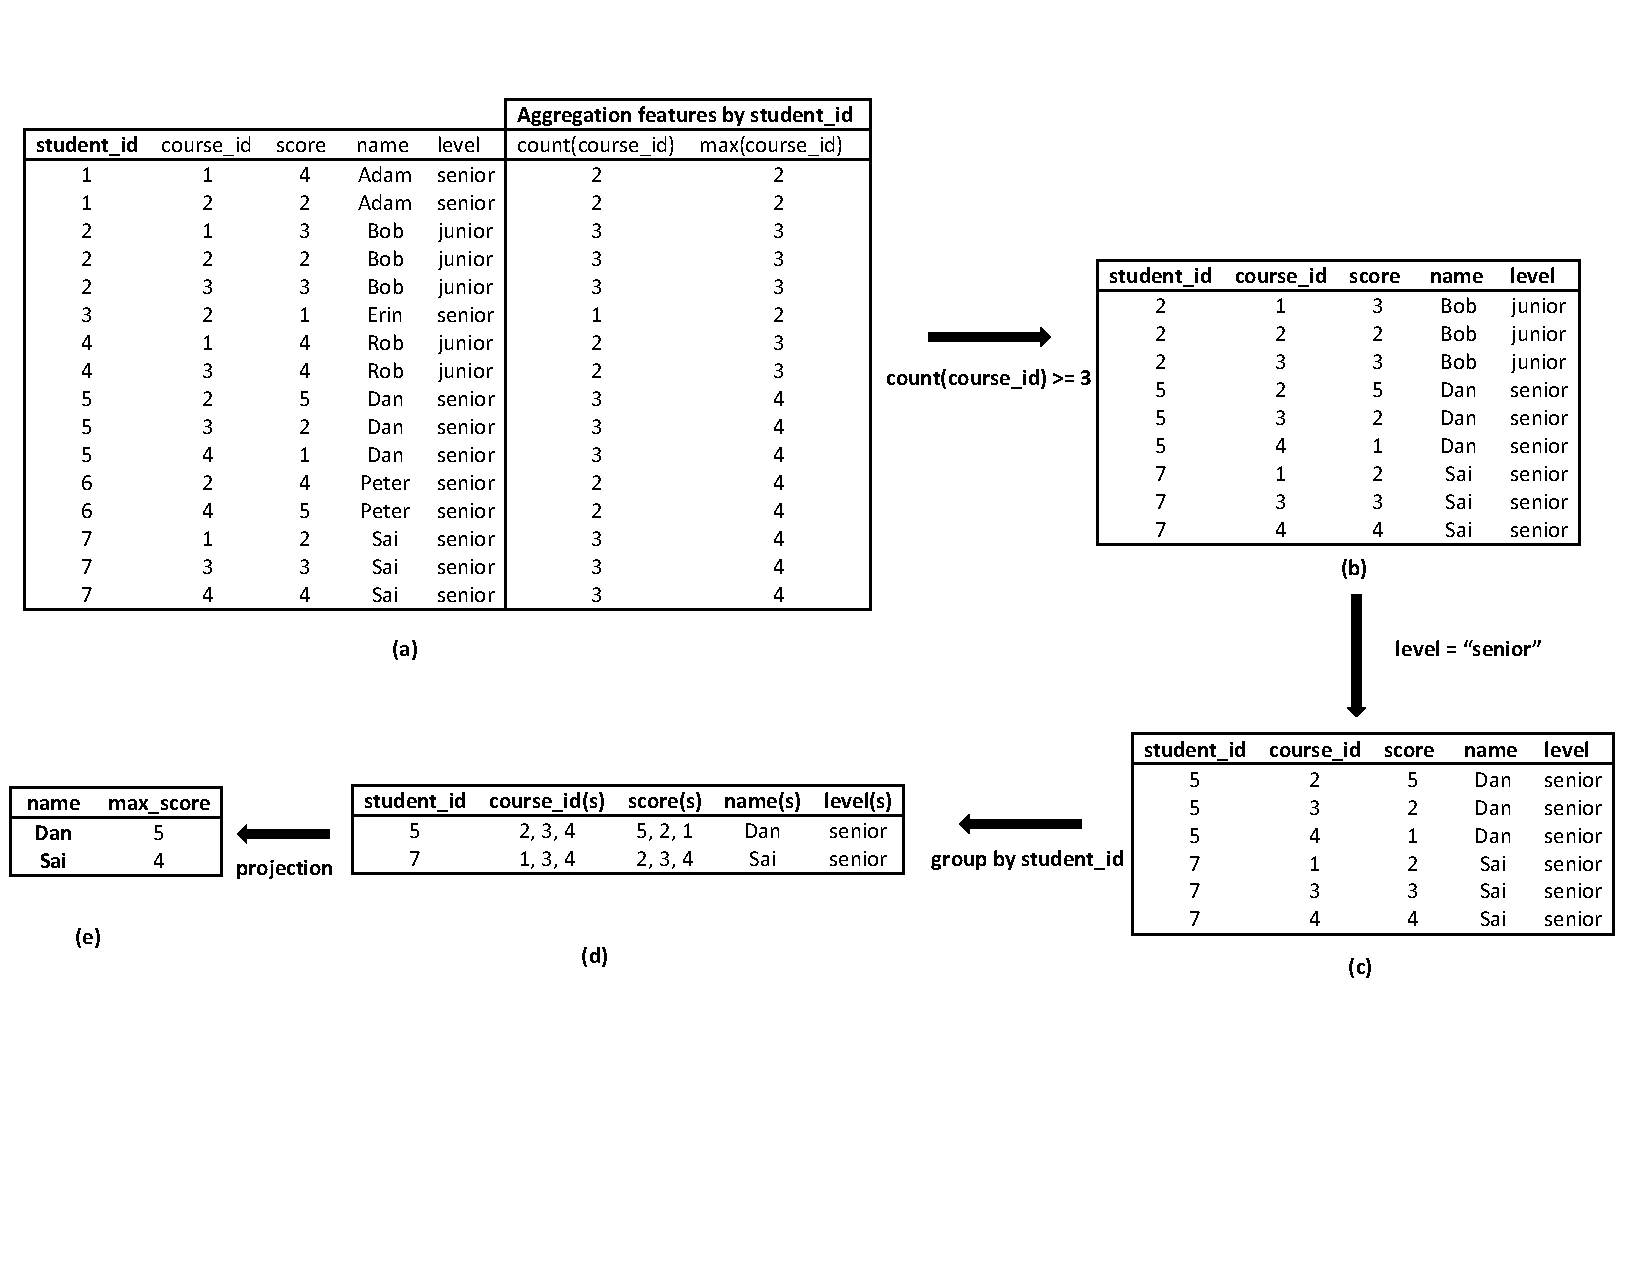
\includegraphics[scale=0.65]{fullexample}
  \vspace*{-1.0ex}\caption {{\label{fig:fullexample}
  Illustration of xxx 
}}

\end{figure*}

In this step, \ourtool takes as input a query skeleton, infers
the missing parts, namely
query conditions (Section~\ref{sec:condition}) and
aggregation operators (Section~\ref{sec:agg_search}); and then produces a
set of syntactically-correct SQL queries.

%The SQL skeleton produced by the first step, though incomplete,
%serves as a good reference in inferring complete and valid SQL queries.
%In this step, our technique the remaining incomplete parts: conditions and
%aggregates, by rule-based learning and type-directed search, respectively.

\subsubsection{Inferring Query Conditions}
\label{sec:condition}

The problem of inferring query \textit{conditions} can be cast as finding
appropriate \textit{rules} that can perfectly divide the whole searching space
into positive part and negative part. In our context, the searching space
contains all tuples generated by joining the input tables, the positive part
are all tuples in the output table, and the negative part are the rest
tuples.

\ourtool uses the PART learning algorithm~\cite{Frank:1998} from
the machine learning community to infer a set of accurate and
expressive rule set. Compared to other well-known learning algorithms
like decision-tree learning or \todo{add}, PART has two
notable features. \todo{unclear}
First, it utilizes the ``divide-and-conquer'' strategy to repeatedly
build rules and remove the instances it covers until no examples are left.
When creating each rule, it employs a pruned decision tree built from
current set of instance and only makes the leaf with the largest coverage
into the resulting rules, without keeping the whole learned tree in memory.

A key challenge in using the PART algorithm is how to devise meaningful
features. Existing approaches~\cite{} simply uses concrete values in a tuple
as features. However, doing so loses much useful structure information
needed in a SQL query.
\todo{not enough, no support for max, min, sum}
Thus, we must transform tuples into appropriate feature representation.

\ourtool addresses this problem by encoding two types of
additional features for each tuple:

\begin{itemize}

\item {\textbf{Aggregation Features}}. Aggregation
features are the aggregation results grouped by each \CodeIn{String} type column
over every other columns. Table~\ref{tbl:agg} shows an example.
(1) Aggregation, including \CodeIn{COUNT}, \CodeIn{MAX},
\CodeIn{MIN} and \CodeIn{AVG}, whose results might be used in query condition.


\item {\textbf{Comparison Features}}. Comparison
feature is the result of comparing two comparable columns. We
consider two possible values:  $\{1, 0\}$,  which represents
means whether two columns under comparison satisfy the predicate or not, respectively.
Comparison results between two comparable columns.
The above two additional knowledge encoding permits our technique
to make use of correlations between columns, rather than only values
from each isolated and sequential columns.
Table~\ref{tbl:com} shows an example.

%the feature would be $0$. Suppose  the comparison features
%for them are summarized in Table \ref{tbl:com}.

\end{itemize}

\vspace{1mm}



\begin{figure}[t]
	\begin{center}
		\begin{tabular}{|c|c|}
		\hline
		\textbf{group by}	& \textbf{aggregation} \\
		\hline
		$C_1$ 				& \textsf{COUNT}($C_2$), \textsf{MAX}($C_3$), \textsf{MIN}($C_3$), \textsf{AVG}($C_3$)\\
		$C_2$ 				& \textsf{COUNT}($C_1$), \textsf{MAX}($C_3$), \textsf{MIN}($C_3$), \textsf{AVG}($C_3$)\\
		\hline
		\end{tabular}
	\end{center}
	\caption{The generated aggregation features for
a table with 3 columns:  $C_1$, $C_2$, and $C_3$, in which
columns $C_1$ and $C_2$ are \textsf{String} type and column $C_3$ is
\textsf{Integer} type.}
	\label{tbl:agg}
\end{figure}



\begin{figure}[t]
	\begin{center}
		\begin{tabular}{|c|c|}
		\hline
		\textbf{predicate}	& \textbf{comparison result} \\
		\hline
		$C_1=C_2$ 			& 0\\
		$C_1<C_2$ 			& 1\\
		$C_1>C_2$			& 0\\
		\hline
		$C_3=C_4$ 			& 1\\
		$C_3<C_4$ 			& 0\\
		$C_3>C_4$			& 0\\
		\hline
		\end{tabular}
	\end{center}
	\caption{The generated comparison features
for a table with 4 columns: $C_1$, $C_2$, $C_3$,
and $C_4$, in which columns $C_1$ and $C_2$ are \textsf{String} type, and
columns $C_3$ and $C_4$ are \textsf{Integer} type. Columns with
the same type are comparable, such as $C_1$ and $C_2$, and
$C_3$ and $C_4$.
}
	\label{tbl:com}
\end{figure}

Combining using concrete tuple values, aggregation
features, and comparison features, our technique is able to
extract expressive feature representation for tuples,
and permits users to encode domain knowledge and structural
information about a SQL query.

\todo{should give an example here of why such feature is useful}


The PART algorithm returns rules representing three types of features.
\todo{which 3 types?}
\todo{move below text to the example figure}
For example, it returns the following rules for our motivating example in Section~\ref{sec:example}:
%. For our
%motivating example there is one rule learned from input tuples. It is

\smallskip
{
\CodeIn{COUNT(enrolled.course\_id) $>$ 2}
}

\CodeIn{\&\& student.level =`senior'}.
%\smallskip

\ourtool next splits the returned rules into two parts: the query selection
condition, and the having condition. 
\ourtool treats rules derived from the value features
as the query conditions (\CodeIn{COUNT(enrolled.course\_id) $>$ 2}
for the example of Figure~\ref{fig:motivating}),
and rules derived from
the aggregation features as the having condition (\CodeIn{\&\& student.level =`senior'}
for the example of Figure~\ref{fig:motivating}). \todo{explain why?}

%To achieve this, we
%use $P_o$ to denote predicates related to original features
%directly derived by the concrete tuple values,
%$P_a$ to denote predicates related to aggregation features and $P_c$ to
%denote predicates related to comparison features. For predicate in $P_o$,
%we use it to fill condition holes in select clause by comparing selected
%column with a constant value. For predicate in $P_a$, we
%can use it to fill aggregation holes in having clause.


%\end{itemize}

\subsubsection{Searching for Aggregation Operators}
\label{sec:agg_search}

For each column produced by an aggregation operator,
the whole search space includes all possible combinations
of table columns and the five supported aggregation operators (see Figure~\ref{fig:syntax}).
\ourtool leverages the following two observations to
further reduce the search space:

\begin{itemize}
\item The data type of an output column must be compatible with the
aggregation operator's return type. For instance, if an output column
has the String type, it must not use aggregation operators (e.g.,
\CodeIn{count} and \CodeIn{sum}) that returns
an Integer. 

\item If an arithmetic aggregation operator, such as \CodeIn{max} and \CodeIn{min},
is used, each value in the output column must has appeared in the input table.
\end{itemize}

%In our experience, the type-directed searching strategy significantly reduces the
%searching space and makes our tool find the desirable aggregates faster.

\todo{Order by structure, relatively each to add}
